\documentclass{article}
\usepackage[margin=0.5in]{geometry}
\usepackage{framed}
\usepackage{graphicx}
\usepackage{wrapfig}
\usepackage{listings}
\usepackage{amsmath, esint}
\usepackage{hyperref}
\usepackage{pdfpages}
\setlength{\parindent}{0cm}
\thispagestyle{empty}
\pagestyle{empty}
\newcommand{\Lagr}{\mathcal{L}}
\newcommand{\AnsLine}{\hspace{0.2 cm} \underline{\hspace{2 cm}}}
\newcommand{\Hgap}{\hspace{0.5cm}}
\newcommand{\Ihat}{\hat{i}}
\newcommand{\Jhat}{\hat{j}}
\newcommand{\Khat}{\hat{k}}
\newcommand{\Xhat}{\hat{x}}
\newcommand{\Yhat}{\hat{y}}
\newcommand{\Zhat}{\hat{z}}
\newcommand{\Nhat}{\hat{n}}
\newcommand{\DEL}{\vec{\nabla}}

\newcommand{\bfemph}[1]{\textbf{\emph{#1}}}

\setlength\parindent{0pt}
\def\changemargin#1#2{\list{}{\rightmargin#2\leftmargin#1}\item[]}
\let\endchangemargin=\endlist 

\title{\textbf{cMag:} A \emph{C} Version of the CLAS12 magnetic field package}

\author{D. Heddle  \\
	\emph{Christopher Newport University}  \\
         \emph{david.heddle@cnu.edu}\\
	}

\date{\today}

\begin{document}

\maketitle
\begin{abstract}
   The standard CLAS12 magnetic field that reads and interpolates the binary field maps for the solenoid and torus was written in JAVA. The package described here reproduces the same functionality in \emph{C}. That's  \emph{C}, not \emph{C++}, 
\footnote{The reason should be obvious. \emph{C} is the most beautiful programming language ever created while, remakably, \emph{C++} is the most hideous. This is not a matter of opinion.\\},\footnote{Pointer arithmetic, fine-grained control over memory (what could go wrong?), a preprocessor that allows you to hide critical code in inpenetrable macros, and a type-unsafe compiler that looks at your line of code that equates an integer pointer to an array of strings and says: ``Ehh, works for me! I assume you know what you are doing." I mean, how can you not love it!\\}
 but of course it can used in a \emph{C++} program. The most important feature is that it reads the same fieldmap files as the JAVA version. The code has been tested on OSX 10.15.4, ubuntu linux 20.04, and one other operating system. \footnote[666]{That would be Windows 10.}


\end{abstract}
\newpage

\section {Introduction}

\section {Where do I get it?}
\subsection {The Code}
Like everything else that isn't available on \textit{Amazon}, the \textit{cMag} distribution is available on github at:
\newline
\newline
\url{https://github.com/heddle/cmag}.
\newline
\newline
\subsection {Field Maps}
An exception to the rule stated above, the field maps are not available on either \textit{Amazon} or github. The field map files are not part of the \texttt{cMag} distribution \footnote{This is because some people are overly sensitive about having gigabytes of field map data stored in every CLAS12-related repository.\\}. They can be downloaded from here:\
\newline
\newline
 \url{https://clasweb.jlab.org/clas12offline/magfield/}.
\newline
\newline

\subsection {File Format}
Provided mostly for completeness, and demonstrating the raw power of \LaTeX, the fieldmap file format document has been inserted starting on the next page. If that doesn't work, the document is also included in the  \texttt{docs} directory of the \textit{cMag} distribution. \footnote{ As, self-rerentially, this document is, referring to the location where it is stored at the location where it is stored.}
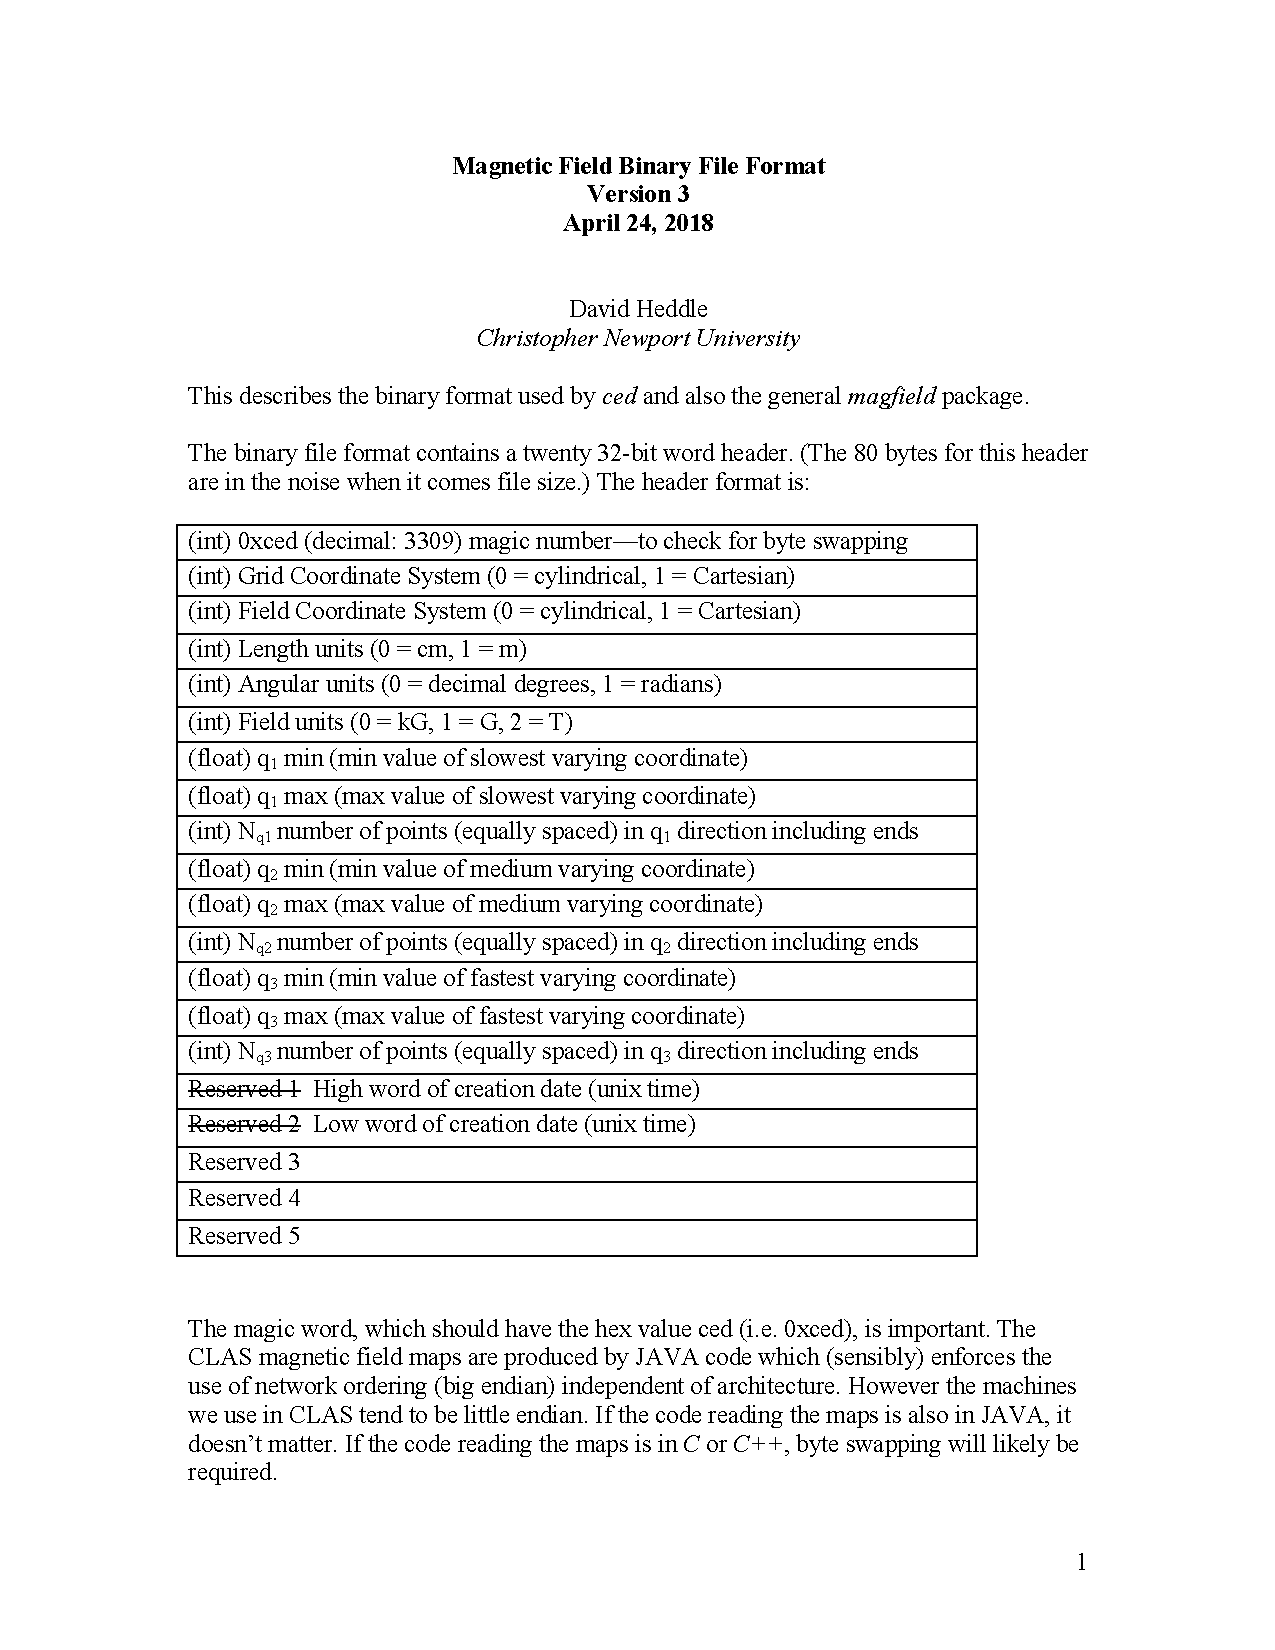
\includepdf[pages=-,pagecommand={},width=\textwidth]{FieldmapFileFormat.pdf}

\section {Building}
After cloning the \textit{cMag} repository, simply work your way down to deepest \texttt{cMag} folder where you will find a \texttt{Makefile}. Now, I have not written a makefile since CLAS was a 6 GeV toddler, but I do seem to recall that they are always very portable and never cause any grief. So I am comfortable that simply typing
\newline
\newline
\textbf{\texttt{\$make all}}
\newline
\newline
will work on any platform. 
\subsection {Testing}
\section {Usage}

\section{Complete API}

\end{document}
